\documentclass[border=1pt]{standalone}
\usepackage[T1]{fontenc}
\usepackage{helvet}
\usepackage[scaled=0.83]{beramono}
\usepackage{tikz}
\usetikzlibrary{arrows.meta,positioning,calc,fit}
\begin{document}
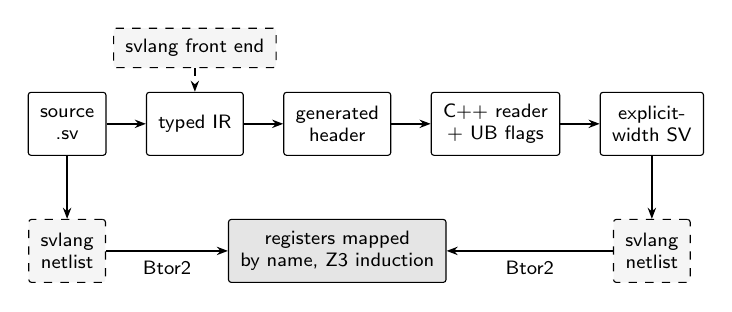
\begin{tikzpicture}[font=\sffamily\scriptsize,node distance=4mm and 5mm,
  box/.style={draw,rounded corners=1pt,align=center,minimum height=8mm,inner xsep=1.5mm,fill=white},
  arr/.style={-{Stealth[length=4pt]},thick},
  sh/.style={draw,dashed,rounded corners=1pt,align=center,minimum height=8mm,inner xsep=1.5mm,fill=black!4}]
\node[box] (src) {source\\.sv};
\node[box,right=of src] (ir) {typed IR};
\node[box,right=of ir] (hpp) {generated\\header};
\node[box,right=of hpp] (rd) {C++ reader\\+ UB flags};
\node[box,right=of rd] (ew) {explicit-\\width SV};
\node[sh,below=8mm of src] (n1) {svlang\\netlist};
\node[sh,below=8mm of ew] (n2) {svlang\\netlist};
\node[box,below=8mm of hpp,fill=black!10] (z3) {registers mapped\\by name, Z3 induction};
\node[sh,above=3mm of ir,minimum height=5mm] (fe) {svlang front end};
\draw[arr] (src) -- (ir);
\draw[arr] (ir) -- (hpp);
\draw[arr] (hpp) -- (rd);
\draw[arr] (rd) -- (ew);
\draw[arr] (src) -- (n1);
\draw[arr] (ew) -- (n2);
\draw[arr,dashed] (fe) -- (ir);
\draw[arr] (n1) -- node[below]{Btor2} (z3);
\draw[arr] (n2) -- node[below]{Btor2} (z3);
\end{tikzpicture}
\end{document}
